
\section{Preliminaries}\label{sec:pre}

Graph representation learning has been a topic of extensive research over the past few decades. This journey, illustrated in Figure~\ref{fig:pre1}, has witnessed the evolution from shallow embedding methods to supervised graph neural networks, transitioning from the fine-tuning paradigm to the emerging prompting paradigm. In this section, we will provide an overview of the fundamental notations employed in this survey, delve into the historical developments of graph representation learning, explore the pre-training and fine-tuning paradigm, and trace the evolution of prompt-based learning. Most importantly, we will present a novel perspective focusing on flexibility and expressiveness, shedding light on why prompts offer a promising solution to address the limitations of existing graph representation learning methods.


\subsection{Notations}\label{subsec:notation}
Let a graph instance denoted as $\mathcal{G} = \{ \mathcal{V}, \mathcal{E} \}$, where $\mathcal{V} = \{ v_1,v_2, \ldots, v_N \}$ represents the node set containing $N$ nodes. The edge set $\mathcal{E} \in \mathcal{V} \times \mathcal{V}$ describes the connection between nodes. Each node $v_i$ is associated with a feature vector represented as $\textbf{x}_i \in \mathbb{R}^D$. To characterize the connectivity within the graph, we employ the adjacency matrix denoted as $\textbf{A} \in \{0,1\}^{N \times N}$, where the entry $\textbf{A}_{ij} = 1$ if and only if the edge $(v_i,v_j) \in \mathcal{E}$.


\subsection{Graph Representation Learning}
The last decades have witnessed a notable surge in the development of graph representation learning techniques. These approaches can be broadly categorized into two main branches: shallow embedding methods and deep graph neural networks (GNNs). The shallow embedding approach is centered on mapping nodes into lower-dimensional, learnable embeddings, enhancing their applicability in various downstream tasks, as exemplified by node2vec~\cite{grover2016node2vec} and DeepWalk~\cite{perozzi2014deepwalk}. On the other hand, the deep GNNs maintain the input node features as constants and optimize deep graph model parameters for specific tasks, leading to more expressive representation capabilities, as seen in methods such as Graph Convolution Networks (GCN)~\cite{niepert2016learning} and GraphSAGE~\cite{hamilton2017inductive}.


Shallow embedding approaches make input node features learnable parameters, aiming at encoding nodes in a manner that retains the original network's similarity structure. 
According to node similarity definition, these methods can be categorized as factorization-based~\cite{
% belkin2001laplacian, 
% ahmed2013distributed, 
% cao2015grarep, 
ou2016asymmetric, zhang2019prone} and random walk approaches~\cite{grover2016node2vec, perozzi2014deepwalk, wang2019hyperbolic, wang2022common}. 
Despite the flexibility that shallow embedding methods offer for various downstream tasks, they are constrained by their inability to generate embeddings for nodes not encountered during training. Additionally, these approaches lack the capability to incorporate node features. Therefore, more ``deeper" methods, specifically those based on graph neural networks, have been developed to address these limitations.



Most deep GNNs follow a message-passing schema and use a more complex encoder, resulting in powerful expressiveness in graph representation. The representative neural network structure is convolutional graph neural networks (ConvGNNs), which comprise spectral~\cite{defferrard2016convolutional,he2021bernnet}
and spatial methods~\cite{
% atwood2016diffusionconvolutional, 
niepert2016learning, hamilton2017inductive, 
% gao2018largescale, 
velickovic2018graph, shi2021masked, xu2018how}.
While these methods have exhibited remarkable capabilities in various graph-based applications, their reliance on task-specific supervision imposes constraints on their adaptability and generalizability, particularly when dealing with tasks that have limited labeled data. 



In summary, shallow embedding methods offer flexibility, preserving network structure and node content for straightforward graph analytic tasks. However, they lack expressiveness and the ability to encapsulate additional node features. Conversely, GNNs provide more expressive graph representations but require task-specific training data, limiting their transferability. Hence, it calls for a graph learning mechanism that combines expressiveness and flexibility. This need led to the development of the pre-training and fine-tuning paradigm.




\begin{figure}[!t]
    \centering
    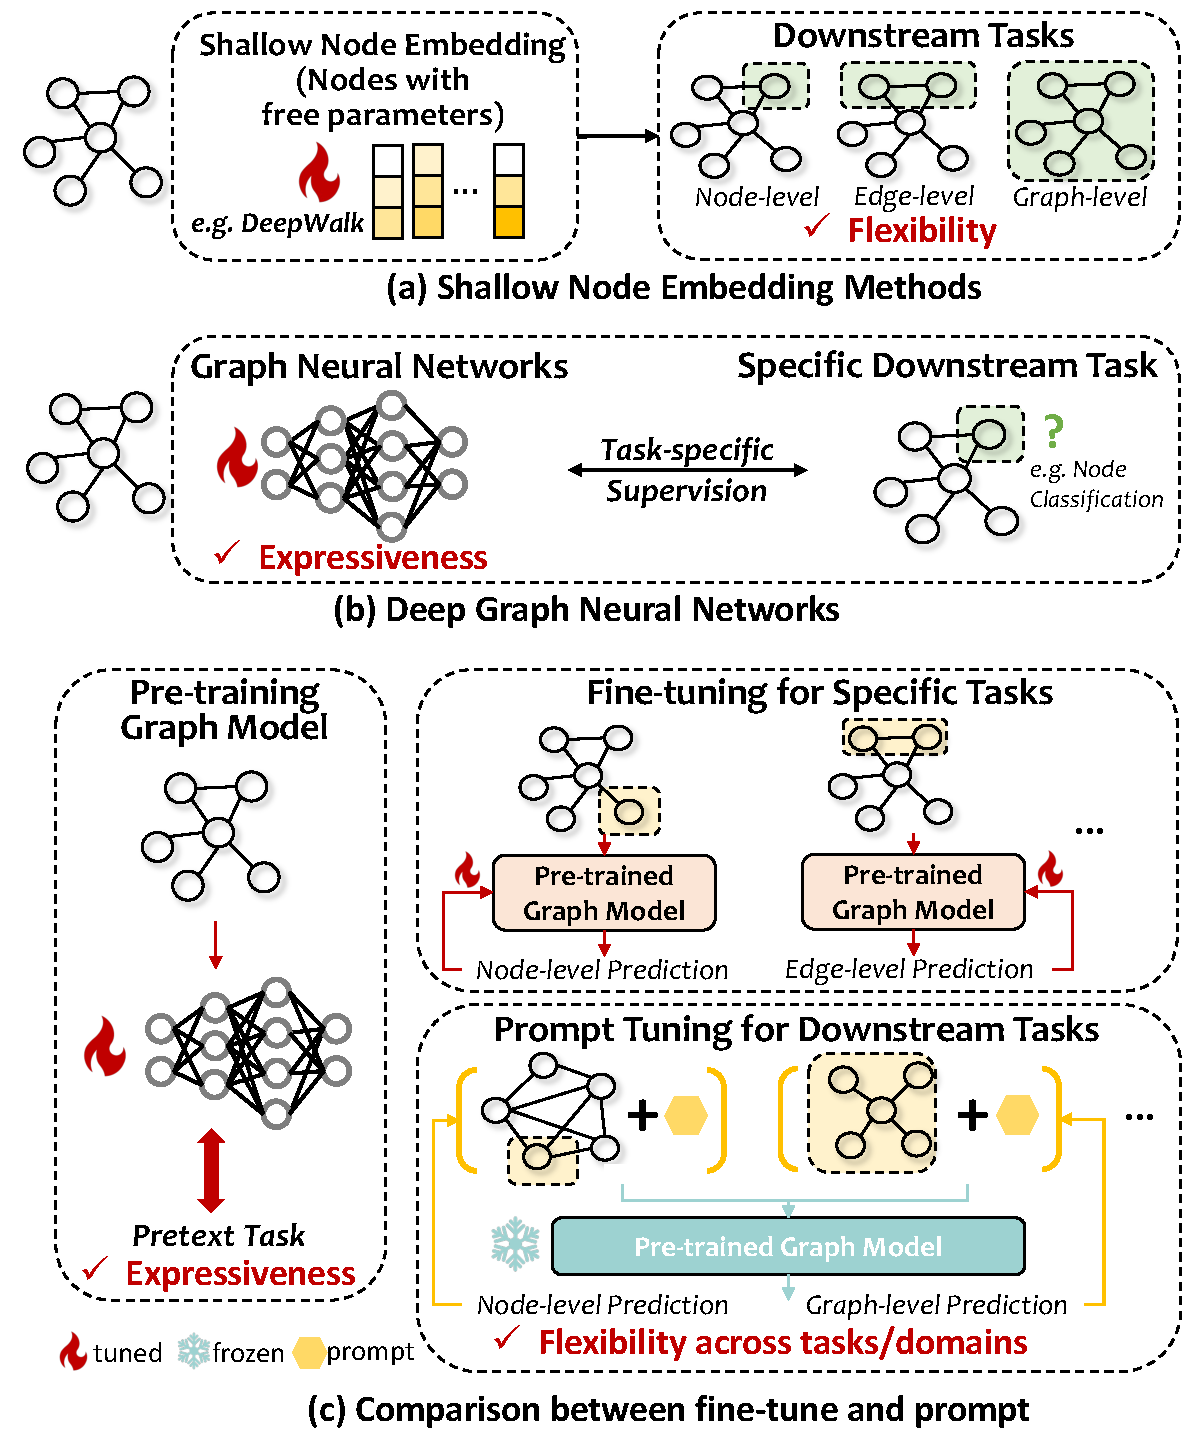
\includegraphics[width=0.49\textwidth]{pic/WhyPrompt2.pdf}
    \caption{Our perspective of prompt upon flexibility and expressiveness. (a) Shallow node embedding methods offer flexibility across different downstream tasks but sacrifice expressiveness. (b) GNNs provide expressiveness but require task-specific supervision and constant node features, limiting their flexibility. (c) Prompts enable a balanced approach, achieving both flexibility and expressiveness.}
    \label{fig:pre1}
\end{figure}

\subsection{Pre-training and Fine-tuning}
To address the challenges of limited labeled data and generalization issues in GNNs, the pre-training and fine-tuning paradigm, thriving in the natural language processing (NLP) community, has gained widespread adoption in graph representation learning. These approaches involve pre-training models on large-scale graph data, with or without labels, followed by fine-tuning model parameters for diverse downstream tasks. This two-step process improves model initialization, yielding broader optima and enhanced generalization compared to training from scratch. Commonly employed pre-training schemes include Graph AutoEncoders (GAEs)~\cite{
% kipf2016variational, 
wang2017mgae}, Masked Components Modeling (MCM)~\cite{hu2020strategies, rong2020selfsupervised}, Graph Contrastive Learning (GCL)~\cite{velickovic2019deep, sun2020infograph}, etc. In Section~\ref{sec:pretrain_method}, we will delve into a detailed discussion of the pre-training and fine-tuning method, offering a comprehensive picture.



\subsection{A Brief History of Prompt Learning}\label{subsec:his_prompt}

Due to the growing number of model parameters, the conventional ``pre-training and fine-tuning`` process is evolving into a new approach termed ``pre-training, prompting, and predicting``~\cite{liu2023pretrain}. In this paradigm, instead of manually adapting the pre-trained model for specific downstream tasks, these tasks are reformulated to resemble those addressed during the pre-training phase, aided by prompts.
Prompts in NLP take various shapes, including cloze prompts
% ~\cite{
% % cui2021templatebased, 
% petroni2019language}
, which complete textual strings like those used in masked language models, and prefix prompts~\cite{lester2021power,li2021prefixtuning}, where the input text precedes the answer slot, as employed by autoregressive language models. Some studies involve manually designed templates based on human insights~\cite{
% petroni2019language, 
brown2020language,schick2021fewshot,schick2021it}, while others explore automated template learning. This includes searching for templates in a discrete space~\cite{jiang2020how, haviv2021bertese, shin2020autoprompt,gao2021making} or conducting prompting directly in the embedding space~\cite{li2021prefixtuning, lester2021power,tsimpoukelli2021multimodal,qin2021learning}.
Such a paradigm enables a single pre-trained model to address a multitude of downstream tasks in an unsupervised manner, which has been widely demonstrated by large language models. In light of this, the application of prompting techniques in the context of graph-based tasks is currently an area of active exploration.


% \subsection{Why Prompt? A New Perspective upon Flexibility and Expressiveness.}\label{subsec:why_prompt}


% Why is prompt learning promising for the graph domain? An existing perspective that appears in most related work is that prompt can reformulate downstream tasks to the pre-training task, which might fill the gap between them. This perspective is good but still not profound enough to see the intrinsic difference from traditional fine-tuning. For example, in a similar perspective, pre-training and fine-tuning can be treated as using fine-tuning to reformulate the pre-training task to the downstream task. It seems that these two technique routines can both address the same problem. Why the first choice is better than the second one?


% In this section, we propose a new perspective, from this view, we can further see the difference between prompting and fine-tuning. As discussed in previous sections, existing graph representation learning methods fail to achieve a satisfactory trade-off between expressiveness and flexibility. Shallow graph embedding approaches offer flexibility as they can be applied to a wide range of downstream tasks. However, they sacrifice expressiveness due to limited parameterization and the inability to incorporate original node features. Take the DeepWalk model as an example, shallow graph methods usually treat node representations as free parameters, which is very flexible because each node can learn its individual representations independently. However, for the reason of gradient, they can not rely on more complicated networks later, which might lose some expressiveness. Actually, there are many more advanced works with deep graph layers using the node representations from DeepWalk as their input features as these node representations are very general in various tasks. On the other hand, GNN-based methods treat node embedding as constant features and seek to find a powerful network for mapping node features to a specific task, which is very expressive. However, the learned feature transform pattern is applied to all the nodes, which means the model can not treat each node embedding as free parameters, and can not achieve as flexible results as the previous ones. When we have multiple tasks, we usually need to train different versions of the same GNN model, which is not as flexible as the previous one.

% With the above analysis, we can find that traditional fine-tuning actually seeks to further improve the expressiveness of a new task with the pre-trained graph model and can not take care of node flexibility. Unlike fine-tuning, a graph prompt usually has several tokens with free parameters, which is very similar to shallow graph methods. In the meantime, each node in the original graph has constant features for GNN models. By inserting the prompt graph to the original graph, the combined graph has both nodes with constant features and tokens with free parameters. The token parameters can be efficiently tuned, preserving node flexibility. The combined graph is sent to a frozen pre-trained GNN model to leverage the powerful expressiveness of deep graph models.


% In this paper, we argue that the prompting mechanism offers a promising solution to address the limitations of existing graph representation learning methods, effectively balancing flexibility and expressiveness. Pre-trained GNNs inherently possess knowledge of both structural and semantic aspects, enabling the desired level of expressiveness. By introducing prompts, we can seamlessly apply powerful pre-trained models to diverse downstream tasks across various domains in an efficient manner. This is achieved by aligning the format of downstream tasks with that of pre-trained tasks, thus leveraging the full potential of pre-trained models even with minimal supervision signals. While the fine-tuning mechanism can also facilitate domain or task adaptation of pre-trained graph models, it often necessitates a considerable amount of labeled information and requires exhaustive re-training of the pre-trained model. In comparison, the prompt mechanism offers a higher degree of flexibility and efficiency.


\subsection{Why Graph Prompt?}\label{subsec:why_prompt}

% In this part of our study, we aim to understand why prompts are important. We want to uncover the fundamental aspects of graph prompts. What exactly do graph prompts do in graph problems? How do they fit into the complex graphs, and how do they help us achieve the broader goal of creating AI systems that can handle graph data effectively? These questions highlight the significant role that graph prompts play in shaping the future of AI when dealing with graph information.


\textbf{A. Differences between Graph Prompting and Graph Fine-tuning.}
Compared with traditional ``graph pre-training and fine-tuning``, which aims to adjust pre-trained graph models for downstream tasks, ``graph pre-training and prompting`` aims to reformulate downstream tasks as the pertaining task by manipulating input data with graph prompts. In this way, the pre-trained model does not need to be adjusted. A notable difference between graph fine-tuning and prompting is that the former is the training trick on model-level  but the latter simulates various transformation strategies on data level. 

% From the whole picture of AIG, there are many techniques for model-level consideration (like model structure design, training, tunning, etc.) Intuitively, these model-level tricks are more like an iceberg on the surface, while the underwater part, that is data, still heavily relies on some primitive hand-crafted work. Compared with the model-level technique, we have very limited learnable approaches to help us handle data-level issues. Graph prompting is just a very notable choice.  

\textbf{B. Capability of Making Data Manipulation Learnable.}
As demonstrated by many works \cite{fang2022prompt, sun2023all}, graph prompts are effective in simulating various graph transformations (e.g. node, edge, graph removing or adding, and some node feature operations). For example, let $\varphi^*$ be a fixed pre-trained graph model, $\mathcal{G}$ and $\mathcal{G}_p^*$ be the original input graph and prompt graph respectively, $\psi(\mathcal{G}, \mathcal{G}_p^*)$ be the hybrid graph integrated by the original graph and the prompt graph. Let $\mathbf{g}(\mathbf{A}$ be the adjacency matrix, and $\mathbf{X})$ be the future matrix of graph nodes. We use $\mathbf{g}(\mathbf{A}, \mathbf{X})$ to denote various graph transformations, then we have the following equation: 
\begin{equation}\label{equ:error_bound_new}%\vspace{-0.05in}
    \varphi^*\left(\psi(\mathcal{G}, \mathcal{G}_p^*)\right)=\varphi^*(\mathbf{g}(\mathbf{A}, \mathbf{X}))+O^{*}_{p\varphi}
\end{equation}
where 

\textbf{C. Broader Impact than Fine-tuning.}
The capability of data manipulation of graph prompts make it be more potential to more application beyond task transferring like fine-tuning. For example, [] use graph prompts to harmony homophilic and heterophilic graphs, make them as one to learn.  [] use graph prompt to complete broken ppi to help reseraches ... Beyond this, the inner machnise of graph prompt is very similar to text, image prompt, which means it is potential to unify multi-modal data in one way. Data quality estimation, OOD problem etc.

In summary, if we 
